
\newpage 

------------------------------------------------------------------------


\fd{from here - old text --------------}
\section{Experimental Evaluation - text from 'Paxos Gossip' - here to remember aspects to discuss - should be deleted}
\subsection{Topology - from paxos gossip}

The topology of the network interconnecting the processes,
and in particular the latencies between the coordinator and the remaining processes, 
affects the performance of Paxos.
In fact, since the decision of a value requires a round-trip from the
coordinator to a majority of processes, the median of RTTs from the coordinator
to other processes ultimately defines the latency of a Paxos instance.
In the Baseline setup, as the coordinator is directly connected to every process,
the expected median RTT is 178ms, which corresponds to a round-trip from the
coordinator's region (North Virginia) and the seventh region presented in
Table~\ref{tab:wan} (Frankfurt).

In the Gossip and Semantic Gossip setups, as the coordinator is not directly
connected to all processes, it interacts with most of them via multi-hop
communication paths.
As a result, the expected RTT from the coordinator to a majority of processes
depends on how ``close'' to them the coordinator is in each randomly generated
network overlay.
%
Figure~\ref{fig:topos} illustrates how the expected median RTT can vary in a
system with 105 processes, and the impact of distinct network overlays on
latencies in the Gossip and Semantic Gossip setups with 1KB values under the
same workload.
Results were obtained from 100 randomly generated network overlays, classified
by their expected median RTT (x axis).
The circles in Figure~\ref{fig:topos} highlight the results in the overlay
network adopted in the previously presented experiments, which has an expected
median RTT of 244ms. 



The first observation we can derive from Figure~\ref{fig:topos} is that there
is a correlation between the metric used to represent distinct network
overlays, the expected median RTT, and the measured latencies.
The correlation is more noticeable in the Semantic Gossip setup, for which it
is almost linear.
%
In the Gossip setup, although the trend is also observed, small variations in
the expected median RTT can have relevant impacts on latency.
%
A reason for this behavior is that the adopted metric reflects the
interaction of the coordinator with a majority of processes, while for the
remaining ones this interaction may encompass, depending on the network
overlay, more communication hops and higher latencies.
We observe here the same effect discussed in Section~\ref{sec:cdfs}: the
adoption of the proposed semantic extensions reduces latency variability, and
so also average latencies.

\begin{figure}[]
\centering
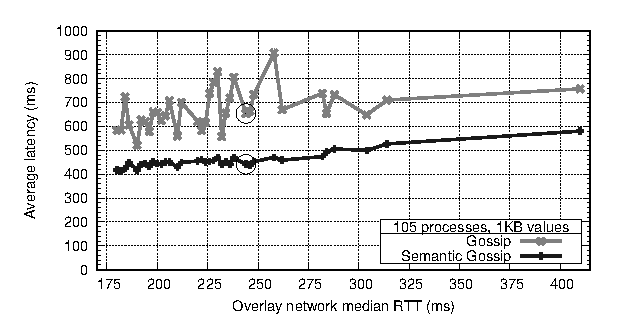
\includegraphics[width=\columnwidth]{figures/lat-rtt.eps}
\caption{Impact of multiple random network overlays on the latency of Paxos in
	Gossip and Semantic Gossip setups.}
\label{fig:topos}
\end{figure}

We also observe that the gains in performance provided by Semantic Gossip are
not related to the option for a given randomly generated network overlay.
In fact, for all random network overlays considered in Figure~\ref{fig:topos}, 
Semantic Gossip improves latency from 25\% to 93\%, 47\% on average, when
compared to the Gossip setup.
While in the network overlay considered in the previously presented
experiments, the improvement in the same configuration was of 32\%.


\subsection{System setup - from paxos gossip}


To provide a fair comparison of results, for each system size $n$, we enforce
the same network overlay in experiments with Gossip and Semantic Gossip setups.
%
In Section~\ref{sec:topos}, we then consider multiple randomly generated
network overlays and argue that this choice does not affect our conclusions.

%As previously mentioned, the average number of peers per process is around
%$2k$, which is also the median of the distribution of peers per process.

We conducted experiments in an emulated WAN, where wide-area latencies were
configured using the Linux Traffic Control kernel module~\cite{ltc}, that
allows postponing the sending of messages to a given destination for a provided
delay.
%
This provided a reasonable and affordable approximation of a large-scale and geographically distributed system with full control of the experiments.
%% https://lartc.org/howto/index.html
%% https://lartc.org/lartc.html#LARTC.QDISC
The injected latency, namely the configured queueing delay, is not fixed but
includes a random jitter of 5\% of the latency.
%
We emulated 13 AWS regions:
%\footnote{\url{https://aws.amazon.com/about-aws/global-infrastructure/regions_az/}}:
North Virginia, Canada, Northern California, Oregon, London, Ireland,
Frankfurt, S\~{a}o Paulo, Tokyo, Mumbai, Sydney, Seoul, and Singapore.
Latencies between AWS regions were extracted from~\cite{crain18}.
%
We have placed the Paxos coordinator in North Virginia in all experiments
because it is the region that has the lowest latency to and from all other
regions.
Table~\ref{tab:wan} lists the WAN latencies between the coordinator's region
(North Virginia), and the other twelve emulated regions.

Clients generate an experiment workload by proposing values to Paxos.
There is one client per region that submits values to a Paxos process hosted
in the same region as the client.
The communication between clients and Paxos processes is reliable.
%
When a Paxos process receives a value from a client, it forwards the value to
the coordinator; the coordinator then proposes the client value in Phase 2 of
the next unused Paxos instance.
%
Paxos processes inform all connected clients about Paxos decisions, although
only value identifiers and instance numbers are sent.
%
When a client is notified of the decision of a value it has submitted, it
computes the end-to-end latency; throughput is computed as the rate of
decisions per time unit.
%
Clients operate in an open-loop model: a client does not wait for the decision
of a submitted value before submitting a new one.
The rate at which clients submit values to Paxos is an experiment parameter,
and all clients submit values at the same rate.

We carried out the experiments in a cluster with two groups of machines: (i)
Dell PowerEdge 1435 with two Dual-Core AMD Opteron 2GHz and 4GB of RAM, and
(ii) HP SE1102 with two Quad-Core Intel Xeon 2.5GHz and 8GB of RAM.
%% 27 machines (i) hosting a single replica each + 13 for clients
%% 39 machines (ii) hosting two replicas each
Due to the lack of sufficient machines for some large-scale experiments, nodes
of group (ii) hosted two processes.
The computational power of each process was of 4 vCPUs with 4GB of RAM,
comparable to {\em xlarge} instances provided by Amazon
EC2.\footnote{\url{https://aws.amazon.com/ec2/instance-types/}}
%% https://ec2instances.info
Machines of each group are connected to two HP ProCurve Gigabit 2920-48G
switches, with 0.1 msec of round-trip time, interconnected by two 10Gbps links.

\subsection{Overall performance - from paxos gossip}

\begin{figure}[!htbp]
\centering

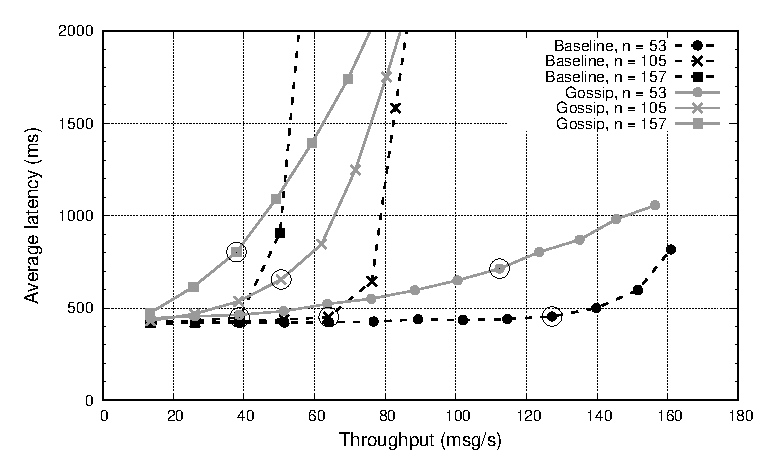
\includegraphics[width=\columnwidth]{figures/lat-th-n-star-gossip.eps}
\caption{Baseline {\em vs} Gossip setups, 1KB values.}
\label{fig:n-b-g}
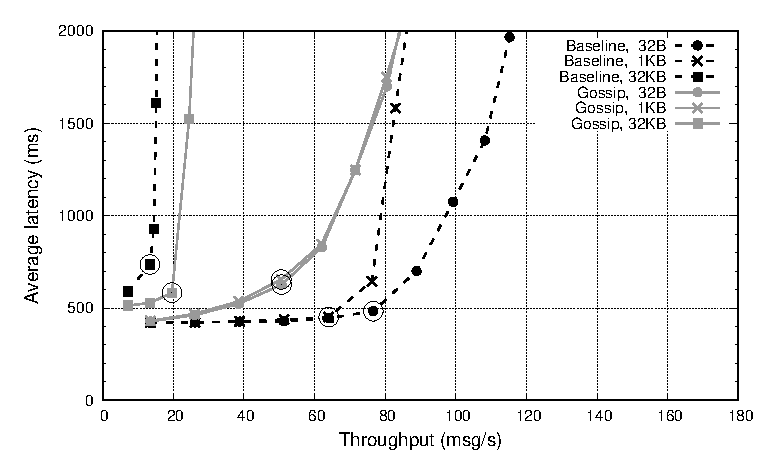
\includegraphics[width=\columnwidth]{figures/lat-th-size-star-gossip.eps}
\caption{Baseline {\em vs} Gossip setups, 105 processes.}
\label{fig:s-b-g}

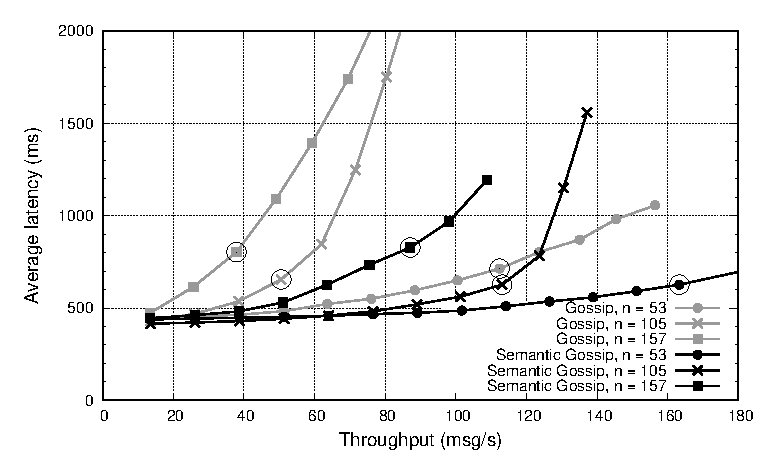
\includegraphics[width=\columnwidth]{figures/lat-th-n-gossip-semantic.eps}
\caption{Gossip {\em vs} Semantic Gossip setups, 1KB values.}
\label{fig:n-g-s}

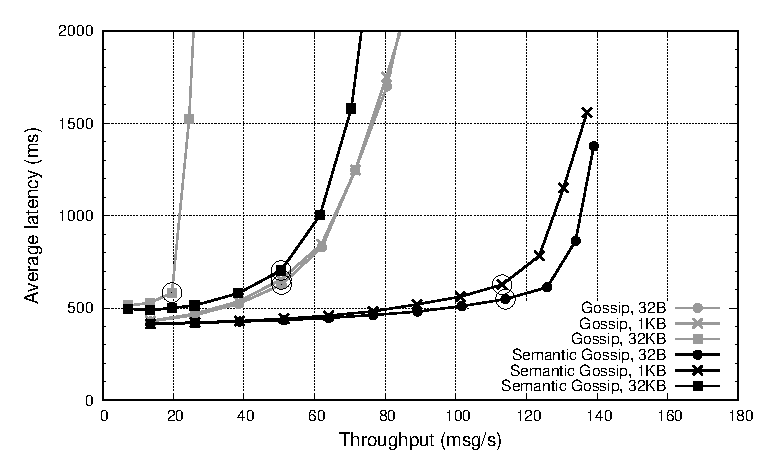
\includegraphics[width=\columnwidth]{figures/lat-th-size-gossip-semantic.eps}
\caption{Gossip {\em vs} Semantic Gossip setups, 105 processes.}
\label{fig:s-g-s}
\
\caption{Throughput vs. latency of Baseline, Gossip and Semantic Gossip.}
\label{fig:overall}
\end{figure}

Figure~\ref{fig:overall} compares the performance of Paxos in the three setups:
Baseline, Gossip, and Semantic Gossip.
%
We varied the number of Paxos processes ($n$), and the size of values clients
submitted to Paxos.
%
In all experiments, the load is generated by 13 clients, one per region, that
submit values at a fixed rate.
%
We subjected Paxos to increasing client workloads until we noticed that the
algorithm is saturated.
%
We highlight the saturation points in the graphs by drawing a circle around
them.
More precisely, for each setup, system size and submitted values size, we
highlight the point of the highest ratio between average latency and throughput.
%
From this point on, increasing client workloads results in small throughput
increments at the cost of relevant latency increments.
%
Throughputs in the saturation points for each system and values sizes are
summarized in Figure~\ref{fig:throughput}.

The graphs on the left of Figure~\ref{fig:overall} (Figures~\ref{fig:n-b-g}
and~\ref{fig:n-g-s}) evaluate the scalability of Paxos in the three setups.
We fixed the size of submitted values to 1KB and varied the number of
Paxos processes: $n$ = 53, 105, and 157.
These system sizes were obtained by placing, respectively, 4, 8, and 12
processes in each of the 13 regions.
An additional process, which acts as the Paxos coordinator, is placed in North
Virginia region, so that the system size $n$ is always odd.
%
The graphs on the right of Figure~\ref{fig:overall} (Figures~\ref{fig:s-b-g}
and~\ref{fig:s-g-s}) evaluate the performance of Paxos in the three setups when
we vary the size of the values proposed in consensus.
The system size was fixed to $n$ = 105 processes, and the performance with the
reference value size of 1KB is compared against the performance with 32B values
and 32KB values.

\subsubsection{Baseline versus Gossip}
\label{sec:basevsgossip}

The graphs at the top of Figure~\ref{fig:overall} compare the performance of
Paxos in the Baseline and Gossip setups.
The first conclusion we draw from Figure~\ref{fig:n-b-g} is that the
Baseline setup provides lower latencies than the Gossip setup for all system
sizes, at least to the saturation points.
Considering the lowest client load at which the algorithm saturates for each
system size, the average latency in the Gossip setup is from 49\% to 79\% higher
than in the Baseline setup.
%% Lowest saturation loads: Gossip x Baseline
%% n = 53, 9 msg/s: 713.111ms x 439.859ms (62,1%)
%% n = 105, 4 msg/s: 654.375ms x 437.783ms (49,5%)
%% n = 157, 3 msg/s: 802.894ms x 448.784ms (78,9%)
%
The inherent cost of epidemic dissemination, multi-hop communication and higher
message complexity is noticeable.
%
Also in terms of throughput at the saturation points, the Baseline setup
outperforms the Gossip setup in all system sizes.
It is worth noting, however, that with 157 processes saturation throughputs are
quite close, despite the relevant gap between latencies.

When we vary the size of submitted values, we observe two distinct scenarios,
depicted in Figure~\ref{fig:s-b-g}.
While the Baseline setup presents better results with (small) 32B values, the
Gossip setup outperforms the Baseline setup with (large) 32KB values.
%
In the Baseline setup, the coordinator sends a Phase 2a message containing the
proposed value to every process.
The cost of this operation is directly associated to the number of
Paxos processes and to the size of proposed values.
%
When clients submit 32KB values, the coordinator becomes fully saturated at
low loads; when values are 32 bytes, not only does the algorithm saturate at
higher loads, but the latency degradation after the saturation point is also
smoother.
%
In the Gossip setup, the load of disseminating values is distributed among all
processes.
The overhead of sending or forwarding 32KB values is noticeable, but less relevant than in the Baseline setup.
%
The performance for the cases of 32B values and 1KB values, however, is similar.
We explain this by the fact that communication is not dominated by messages carrying
(full) values, but by Phase 2b and Decision messages that only carry value ids.

\begin{figure*}[htbp]
\centering
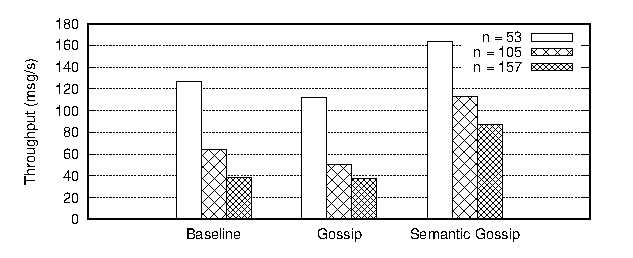
\includegraphics[width=\columnwidth]{figures/throughput-saturation-1kb.eps}
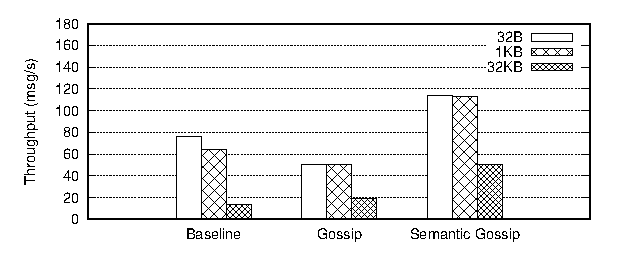
\includegraphics[width=\columnwidth]{figures/throughput-saturation-n105.eps}
\caption{Throughput at saturation point in all setups, with 1KB values (left)
	and with 105 processes (right).}
\label{fig:throughput}
\end{figure*}

An explanation for the lower performance of Paxos in the Gossip setup is the
inherent redundancy of gossip communication.
%
We then compared the average number of messages exchanged, in experiments with
the same load, by the Paxos coordinator in Baseline and Gossip setups.
In the Baseline setup the coordinator is the only process that
communicates with all processes, thus the most overloaded process.
In the Gossip setup, in terms of communication, the coordinator is a process
like any other.
%
With 105 processes, the number of messages received by a regular process in the Gossip
setup is from 11 to 12 times the number of messages received by the coordinator
in the Baseline setup.
As we do not expect message duplication in the Baseline setup, the redundancy factor
in the Gossip setup is around 11 times. 
In fact, the gossip layer discards about 91\% of received messages because they
are duplicated.
%
When we vary the system size, the redundancy factor in the Gossip setup is smaller
but still relevant.
%
For $n$ = 53, the redundancy factor is from 4 to 5 times and around 80\% of
received messages are duplicated.
This is due to the smaller number of peers each process has when $n$ is dropped
by half ($log_257 \approx 6$ and $log_2105 \approx 7$).
%
With $n$ = 157, the redundancy factor is around 7 times and duplicated messages
are about 85\%.
%In this case, 
The number of peers per process is the same as with $n$ = 105
($log_2105 \approx log_2157 \approx 7$), but the number of processes is
increased by 50\%.

\subsubsection{Gossip versus Semantic Gossip}
\label{sec:gossipvssgossip}

The graphs at the bottom of Figure~\ref{fig:overall} compare the performance of
Paxos in the Gossip and Semantic Gossip setups.
By extending the gossip-based communication layer with the semantic filtering and
aggregation methods, the performance of Paxos is improved in all
configurations evaluated.
%% Lowest saturation loads: Gossip x Semantic Gossip
%% n = 53, 9 msg/s: 713.111ms x 509.525ms (-28,5%)
%% n = 105, 4 msg/s: 654.375ms x 441.689ms (-32,5%)
%% n = 157, 3 msg/s: 802.894ms x 481.842ms (-40,0%)
Considering the saturation loads for the Gossip setup, Semantic Gossip reduced the
average latencies for 1KB values by 28\%, 32\%, and 40\% with, respectively,
53, 105, and 157 processes (Figure~\ref{fig:n-g-s}).
%% Saturation loads: Semantic Gossip x Gossip
%% n = 53: 13 msg/s, 626.267ms, 163.246 msg/s x 112.377 msg/s (-12,2%, 1.45x)
%% n = 105: 9 msg/s, 626.504, 113.08 msg/s x 50.5732 (-4.3%, 2.24x)
%% n = 157: 7 msg/s, 827.617ms, 87.0696 msg/s x 37.888 msg/s (+3.1%, 2.30x)
In addition, as depicted on the left part of Figure~\ref{fig:throughput},
saturation throughputs are, respectively, 1.45, 2.24, and 2.30 times higher in
the Semantic Gossip setup than in the Gossip setup.
%
Thus, as we scale up the system, the more relevant the benefits of the
semantic extensions in the performance of Paxos are.

%% Lowest saturation loads: Gossip x Semantic Gossip
%% s = 32B, 4 msg/s: 626.922ms x 434.502ms (-30,7%)
%% s = 1KB, 4 msg/s: 654.375ms x 441.689ms (-32,5%)
%% s = 32KB, 1.5msg/s: 583.304ms x 500.996ms (-14,1%)
Varying the size of submitted values (Figure~\ref{fig:s-g-s}), Semantic Gossip
reduces latencies by 31\% with 32B values, and 14\% with 32KB values,
considering the saturation loads for the Gossip setup.
%% Saturation loads: Semantic Gossip x Gossip
%% s = 32B: 9 msg/s, 547.863ms, 114.031 msgs/s x 50.7046 msg/s (-12,6%, 2.25x)
%% s = 1KB: 9 msg/s, 626.504ms, 113.08 msg/s x 50.5732 msg/s (-4.3%, 2.24x)
%% s = 32KB: 4 msg/s, 703.708ms, 50.5082 msg/s x 19.6444 msg/s (+20,6%, 2.57x)
At the saturation point of the Semantic Gossip setup, throughput is 2.25 and
2.57 times higher than the saturation throughputs of the Gossip setup for 32B
and 32KB values, as observed on the right graph of Figure~\ref{fig:throughput}.
%
As the effect of semantic extensions is essentially on the propagation of Phase 2b
messages, that do not include full values, benefits are similar for different
values sizes.
%
In particular, for 32B and 1KB values improvements are identical, resulting in
similar performance in both the Gossip and Semantic Gossip setups.
With 32KB values, the least relevant reduction in average latency with the
adoption of Semantic Gossip was observed (14\%); it is an expected result, as
latencies in this configuration are dominated by the cost of disseminating
large values.
%
The increment of saturation throughput, however, is slighter better (2.57
times), as saving network resources in this configuration is potentially more
beneficial.

The advantage of Semantic Gossip can be explained when we compare the number of
messages exchanged by processes via gossip.
%
For the configuration with 105 processes and 1KB values, the number of messages
received by a process in the Semantic Gossip setup is 65\% lower than in the Gossip
setup.
For this reduction, of about 2.9 times, contribute both the messages discarded
through semantic filtering and multiple messages replaced by a single message
through semantic aggregation.
When only semantic filtering is adopted, about 42\% fewer messages are received.
When only semantic aggregation is adopted, about 44\% fewer messages are
received from the network layer; the content of such messages has been included
in aggregated messages.
%
Semantic aggregation does not impact the number of messages delivered to Paxos,
nor the duplication rate, as messages are disaggregated before duplication
check and delivery.
With the adoption of semantic filtering, the number of messages delivered to
Paxos drops by 3.3\%, while the portion of messages discarded because they are
duplicated is 85\% (versus 91\% in the Gossip setup).
%
The inherent redundancy of gossip communication is thus preserved, just as the
application still operates with a reasonably safe level of redundancy.

\begin{figure*}[htbp]
\centering
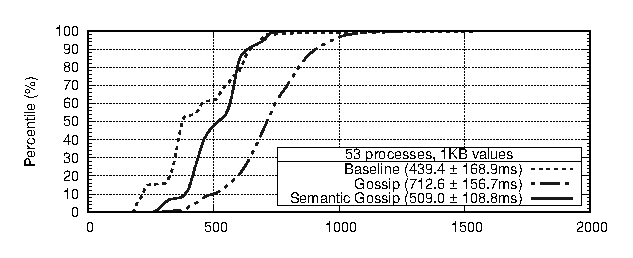
\includegraphics[width=\columnwidth]{figures/cdf-n53-size1kb.eps}
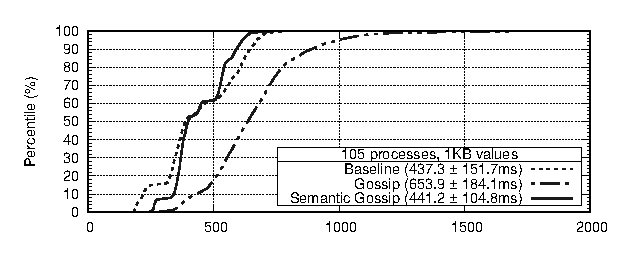
\includegraphics[width=\columnwidth]{figures/cdf-n105-size1kb.eps}
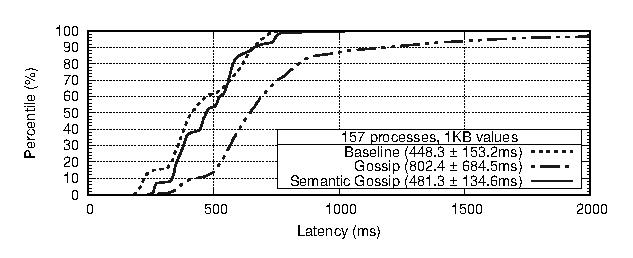
\includegraphics[width=\columnwidth]{figures/cdf-n157-size1kb.eps}
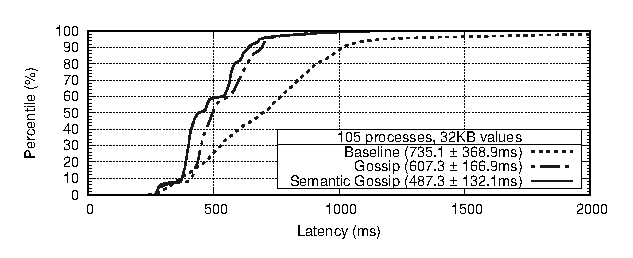
\includegraphics[width=\columnwidth]{figures/cdf-n105-size32kb.eps}
%
\caption{Latency distribution of Baseline, Gossip and Semantic Gossip (legend with average latency and standard deviation).}
\label{fig:cdfs}
\end{figure*}

\begin{table*}
\begin{small}
\setlength{\tabcolsep}{3.5pt}
\begin{tabular}{c|cccccccccccc}
Regions  & Canada & N.California & Oregon & London & Ireland & Frankfurt & S.Paulo & Tokyo & Mumbai & Sydney & Seoul & Singapore \\ \hline
Latency (ms)  & 15  & 64  & 76  & 76  & 85  & 89  & 122  & 162  & 182  & 205  & 209  & 238 \\ 
\end{tabular}
\end{small}
\caption{WAN latencies between the coordinator's region (North Virginia) and the other twelve regions.}
\label{tab:wan}
\end{table*}

\subsection{Latency distributions}
\label{sec:cdfs}

Figure~\ref{fig:cdfs} presents the cumulative distribution function (CDF) of
latencies measured by clients in four configurations for the three analyzed
setups.
Results presented in each graph refer to experiments in which Paxos was
subject to the same client workloads.
%
CDFs on the left explore the behavior at scale, $n$ = 53 and 157 processes,
with 1KB values.
CDFs on the right explore the behavior with $n$ = 105 processes and two value
sizes: 1KB and 32KB; results with 32B and 1KB values are quite similar, so only
the latter are presented.

As observed in Figure~\ref{fig:cdfs}, latency distributions show considerable
dispersion and present several noticeable steps.
This occurs because latencies are measured by 13 clients, one client per
region, that submit a value to a Paxos process located at the same region, then
wait until the corresponding decision is informed by the same process.
The client located at the same region as the coordinator has the advantage of
having its values delivered to the coordinator with low delays.
Latencies measured by this client, about 7.7\% (1/13) of all, are the lowest,
noticeable in the bottom left part of the CDFs, specially in the Semantic Gossip
setup.
Values submitted by clients located in other regions are forwarded to the
coordinator, an operation subjected to WAN latencies.
The cost of this operation is more noticeable in curves for the Baseline setup,
as Paxos processes send values directly to the coordinator.
%
From the second region (Canada) to the coordinator's region (North Virginia)
the latency is relatively small: 15ms---latencies are presented in
Table~\ref{tab:wan}.
The first step in Baseline CDFs is thus around 15.4\% (2/13), following the
latencies measured by clients in the first two regions.
Then, up to the seventh region (Frankfurt), WAN latencies are larger but still
below 100ms.
The step around 53.8\% (7/13) represents this interval, corresponding
approximately to the median of the latency distributions in the Baseline setup.

%% Latency, average +- standard deviation: Baseline, Gossip, Semantic Gossip
%% 53, 1KB: 439.361 +- 168.875, 712.613 +- 156.699, 509.027 +- 108.776
%% 105, 1KB: 437.279 +- 151.701, 653.876 +- 184.143, 441.178 +- 104.787
%% 157, 1KB: 448.286 +- 153.164, 802.394 +- 684.492,  481.337 +- 134.617
%% 105, 32KB: 735.102 +- 368.879, 607.281 +- 166.874, 487.279 +- 132.062

Latencies observed by a client are less affected by its geographic location in
Gossip and, particularly, in Semantic Gossip than in Baseline.
As a result, the standard deviation of latencies is lower in the Semantic Gossip
setup than in the Baseline setup for all configurations depicted in
Figure~\ref{fig:cdfs}.
And in two configurations, with $n$ = 53 and with 32KB values, standard
deviations are lower in the Gossip setup than in the Baseline setup.
Notice that, except for 32KB values, the lowest average latencies for all
configurations are observed in the Baseline setup; standard deviations are thus,
proportionally, even greater.
%
The least latency variability in gossip-based setups is associated to the
adoption of a randomly generated overlay network.
While processes located in close geographical regions are not necessarily
connected, which increases latency between them, processes farther from the
coordinator are not so significantly penalized.
%
Latencies increase, as the shortest route between a process and the coordinator
is the one used in the Baseline setup.
But for processes farther from the coordinator, the decision of a value can be
anticipated, once Phase 2b messages are broadcast, and not only sent to the
coordinator.
%
In summary, submitting values, which are forwarded to the coordinator, is
faster in the Baseline setup.
Once a value is proposed by the coordinator, decision is faster on gossip-based
setups, despite the location of a process and clients to it associated.

\subsection{Reliability}

A major feature of gossip-based communication is its reliability, which allows
masking link and process failures.
This capability stems from the inherent redundancy of gossip dissemination,
attested by the data collected in our experiments.
Since a message is transported through multiple distinct network paths, a
communication disruption between two processes is less likely to prevent it
from being received by all destinations.
%
In this section, we assess the degree of reliability provided by the Gossip and
Semantic Gossip setups.

We implemented a fault-injection mechanism that randomly discards messages
received by a process.
In addition, the timeout-trigged procedures that enable Paxos to react to
message loss events were disabled.
As a result, Paxos processes, and their associated clients, may fail to learn
the decision value for one or some consensus instances.
When any client fails to learn the value decided in any instance of consensus,
we say that the experiment failed.

%We focus our analysis on the Gossip and Semantic Gossip setups, as in the Baseline setup
%injecting a minor rate of message loss causes experiments to fail.
%An experiment fails when a client is not notified about the decision of a value
%it has proposed.
%%
%In the Baseline setup, if a process fails to receive a Phase 2a or a Decision
%message referring to an instance of consensus, it cannot decide; in
%particular because Phase 2b messages carry value ids (not the full value).
%Moreover, if the coordinator fails to receive a value forwarded by a process,
%the value will never be proposed.
%%
%Practical Paxos implementations circumvent these situations by relying on
%timeouts and retransmission mechanisms.
%As we are investigating the reliability of the communication layer, we do not
%consider those mechanisms.
%%
%The interaction between clients and Paxos processes, however, is not affected by
%injected message loss.

\begin{figure}
%\centering
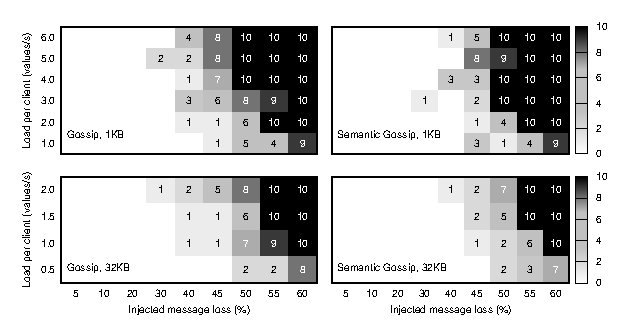
\includegraphics[width=1.02\columnwidth]{figures/heatmap-multiplot.eps}
%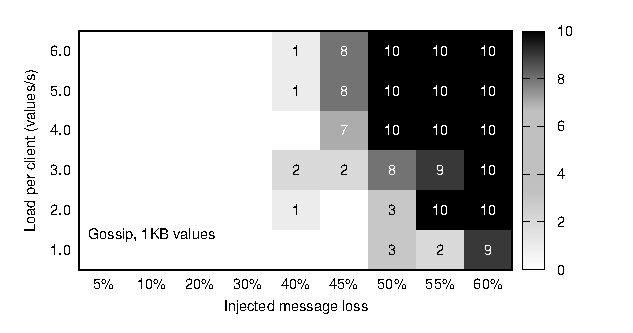
\includegraphics[width=\columnwidth]{figures/heatmap-n105-size1kb-gossip.eps}
%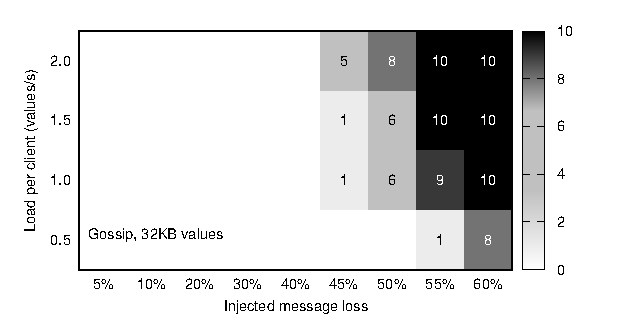
\includegraphics[width=\columnwidth]{figures/heatmap-n105-size32kb-gossip.eps}
%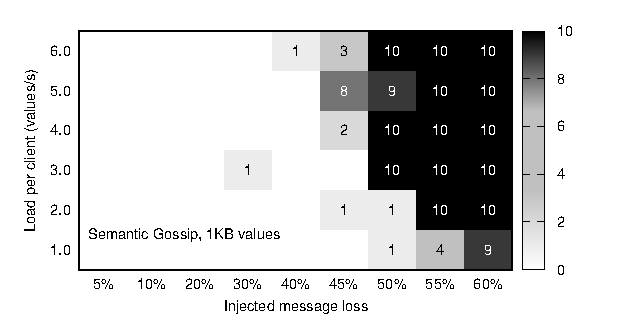
\includegraphics[width=\columnwidth]{figures/heatmap-n105-size1kb-semantic-gossip.eps}
%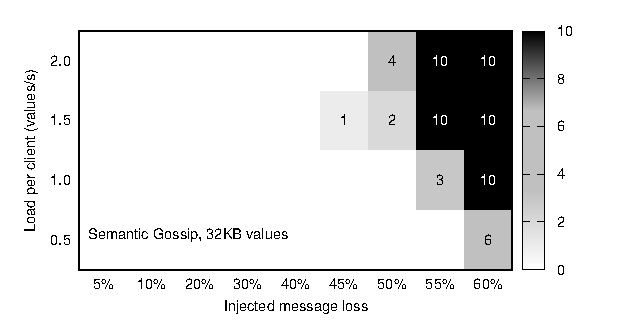
\includegraphics[width=\columnwidth]{figures/heatmap-n105-size32kb-semantic-gossip.eps}
\caption{Number of failed experiments out of 10 attempts in Gossip and Semantic
	Gossip setups under message loss.}
\label{fig:heatmaps}
\end{figure}

Figure~\ref{fig:heatmaps} summarizes the impact of message loss in the
operation of Paxos with 105 processes, 1KB and 32KB values, in the Gossip and
Semantic Gossip setups.
We subject Paxos to increasing workloads, the number of values submitted per second
by each of the 13 clients (y axis), and increasing injected message loss rates
(x axis).
We ran 10 experiments for each client load and message loss rate.
Figure~\ref{fig:heatmaps} depicts the number of {\em failed} experiments.
The white cells of the graph represent configurations for which no experiment
has failed, essentially all configurations subjected to up to 30\% of message
loss.
The black cells, concentrated in the upper right corners (i.e., higher loads
and message loss rates), are configurations for which all 10 experiments have
failed.

We can draw two major conclusions from Figure~\ref{fig:heatmaps}.
%
First, the Gossip setup is indeed resilient to message loss: with 30\% of
injected message loss, the number of failed experiments is very low, 2/60 for
1KB values and 1/40 for 32KB values.
Notice that Paxos is subject to lower workloads with 32KB values, so as not to
saturate the system.
%
Second, the benefits on performance obtained with the adoption of semantic
extensions do not come at the cost of lower reliability.
In fact, the Semantic Gossip setup has proved to be at least as reliable as the Gossip
setup, when considering the overall results.
%
For 1KB values, Semantic Gossip had more failed experiments than Gossip only
under 55\% of message loss (53 vs 54), being better in all others.
For 32KB values, Semantic Gossip had less failed experiments under all message
loss rates, thus a notably better behavior than the Gossip setup.

\begin{figure}[t]
\centering
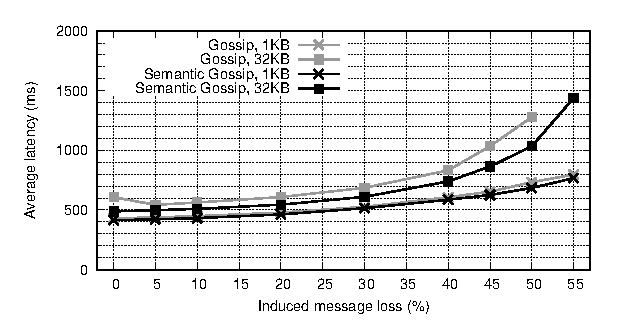
\includegraphics[width=\columnwidth]{figures/msgloss-lat-loss.eps}
\caption{Impact of message loss on the latency of Paxos in Gossip and Semantic
	Gossip setups, with 105 processes.}
\label{fig:msgloss}
\end{figure}

%% Effect of message loss: 0% vs 50%
%% Gossip, 1KB: 733.656 / 430.299 = 1.7049911805511981
%% Semantic, 1KB: 684.932 / 414.773 = 1.6513418182957906
%% Gossip, 32KB: 1278.5 / 607.773 = 2.103581435832128
%% Semantic, 32KB: 1033.59 / 487.77 = 2.119011009287164

%% Effect of message loss: 0% vs 40%
%% Gossip, 1KB: 606.568 / 430.299 = 1.4096430621498075
%% Semantic, 1KB: 585.851 / 414.773 = 1.41246175618953
%% Gossip, 32KB:  831.797 / 607.773 = 1.3685981443729813
%% Semantic, 32KB: 739.686 / 487.77 = 1.516464727227997

Figure~\ref{fig:msgloss} presents the impact of message loss on the average
latency of Paxos in both the Gossip and Semantic Gossip setups.
We only consider configurations for which at least 3 experiments succeeded, and
results refer to a workload of 1 value/s for each of the 13 clients, which
provides similar average latencies in both setups.
%
As we introduce message loss, average latencies tend to increase, and a
corresponding but less noticeable reduction in throughput is also observed.
%
Due to the inherent redundancy of gossip-based communication, messages dropped
by a process are likely to be eventually received again, from another peer.
While this allows information to still be transmitted to all processes, despite
random message loss events, the time it takes for it to be received increases.
The effect on latencies is therefore expected, but reasonably low.
%
With 40\% of message loss, average latencies increase by about 41\% with 1KB
values in both setups.
With 32KB values, the latency increment is of about 37\% in the Gossip and 52\% in
the Semantic Gossip setups.

\subsection{Discussion}

%Table~\ref{tbl:compare} summarizes the main trends in throughput and latency of the Baseline (B), Gossip (G) and Semantic Gossip (SG) setups.
%Throughput relations are computed from the data in Figure~\ref{fig:throughput}; latency relations for average and standard deviation are from Figure~\ref{fig:cdfs}.
%We say that setup A is similar to setup B (A $\sim$ B) if their difference is around 10\%; A is ``better than'' B (A$>$B) is they differ by more than 10\% and one is not twice the other; A is ``much better than'' B if one is twice the value of the other. 
%Finally, A is better than B if A's throughput is higher or A's latency is lower than B's.
%
%\begin{table}[h]
%\small
%\centering
%\begin{tabular}{|l|l|c|c|} \hline
%\multicolumn{4}{|c|}{Throughput} \\ \hline
%1KB		& $n=53$		& \multicolumn{2}{c|}{SG $>$ B $>$ G} \\
%		& $n=105$	& \multicolumn{2}{c|}{SG $>$ B $>$ G} \\
%		& $n=157$	& \multicolumn{2}{c|}{SG $\gg$ B $\sim$ G} \\ \hline
%$n=105$	& 32B		& \multicolumn{2}{c|}{SG $>$ B $>$ G} \\
%		& 1KB		& \multicolumn{2}{c|}{SG $>$ B $>$ G} \\
%		& 32KB		& \multicolumn{2}{c|}{SG $\gg$ G $>$ B} \\ \hline\hline
%\multicolumn{4}{|c|}{Latency} \\ \hline
%		& 			& Average 			& Std deviation \\ \hline
%1KB		& $n=53$		& B $>$ SG $>$ G		& SG $>$ G $\sim$ B\\
%		& $n=105$	& B $\sim$ SG $>$ G	& SG $>$ B $>$ G\\
%		& $n=157$	& B $\sim$ SG $>$ G	& SG $>$ B $\gg$ G \\ \hline
%$n=105$	& 1KB		& B $\sim$ SG $>$ G	& SG $>$ B $>$ G\\
%		& 32KB		& SG $>$ G $>$ B		& SG $>$ G $\gg$ B\\ \hline
%\end{tabular}
%\caption{Trends in relative throughput and latency in Baseline (B), Gossip (G) and Semantic Gossip (SG) under different configurations 
%(A $\sim$ B: $\approx$10\% difference between A and B; A $\gg$ B: A at least 2$\times$ better than B; A$>$B: anything else).}
%\label{tbl:compare}
%\end{table}%

We draw the following main conclusions from our experimental study.
The observations below address each one of the questions that guided our
evaluation (see Introduction).

The adoption of a classic gossip-based communication substrate has, in most
cases, a negative impact on the performance of Paxos.
The higher message complexity and the considerable level of redundancy, which
makes the Paxos coordinator to receive up to 11 times more messages in the
Gossip setup than in the Baseline setup, have an important effect on latency.
Gossip slows down the decision of values, resulting in 49\% ($n$ =
105) to 79\% ($n$ = 157) higher average latencies.
%
A notable exception occurs when proposed values are large (32 KB).
As the load of disseminating full values is distributed among all processes in
the Gossip setup, the coordinator is no longer the system's bottleneck.

Augmenting the gossip-based communication substrate with semantic extensions
significantly improves the performance of Paxos in all configurations
evaluated.
The adoption of semantic filtering and aggregation techniques reduces the number
of messages exchanged by processes via gossip by up to 65\%.
This not only allows Semantic Gossip to provide average latencies typically
30\% lower than in the Gossip setup, but also similar to the latencies in the
Baseline setup.
In terms of throughput, the Semantic Gossip setup is able to sustain higher
workloads, while providing quite low latencies, when compared to both the
Gossip and Baseline setups.
%
Moreover, although most of our results were obtained in a single, randomly
generated, network overlay, we can argue that they can be extended to any
randomly generated network overlay.
%
This consolidates Semantic Gossip as a viable option for the implementation of
Paxos at large scale.

The proposed semantic extensions do not compromise the inherent reliability of
gossip communication.
Our results reveal that the adoption of a gossip-based communication substrate
allows to mask the loss of a considerable portion of messages exchanged by
processes.
In fact, without resorting to any timeout-trigged
retransmission mechanisms, Paxos was able to operate correctly despite 30\% of
message loss, both in the Gossip and Semantic Gossip setups.
%This also shows that by dropping one of the two layers of redundancy achieved
%by executing Paxos atop gossip, the algorithm robustness is preserved.
